\section{Validation and measured performance}
\label{sec:experiments}

The mathematical statements above do not depend on experiment.  The
experiments check that the code implements their hypotheses and conclusions,
that the new source adapter agrees with actual cut manifolds, and that a
claimed kernel improvement survives complete-call measurement.  The
preserved files contain every measured sample, including unfavorable
comparisons and inconclusive cases.

\subsection{Baseline and algebraic validation}

The pinned repository's full native suite passed all 1,663 tests in an
isolated checkout with its original surrounding directory structure.  Its
log also reports 13,846 expanded-sheet topology comparisons.  This is a
baseline check, not a claim that the new modules were already integrated
into that suite.  An initial run from an incomplete copied directory could
not resolve tests' repository-relative fixtures; it was discarded as an
invalid test setup and the full checkout run was used instead.

The column-peeling validation includes the following distinct checks.
\begin{itemize}
\item 31,106 small nonnegative matrices were compared with an independent
recursive search over every allowed positive-pivot order.
\item 600 rectangular cases were checked by separately enumerating
permanent-one full-row minors.
\item 512 binary matrices were checked against the union of all stopping
subsets and against source-order reversal.
\item 24,508 matrices were compared with the pinned minimum-fill planner.
All full-row verdicts agreed, and every successful baseline run used only
zero-fill pivots, as the completeness proposition predicts.
\end{itemize}
These populations overlap and must not be added as if they were disjoint
independent inputs.  Further tests exercise empty rows, empty matrices,
large sparse labels, 4,096-bit counts, inert columns, source immutability,
forged certificates, strict types, and propagated cancellation exceptions.

The relative-bundle tests include an actual layered-solid-torus normal cut
with independent source replay, and separate standard relative topological
models: a saturated disc, M\"obius band, once-punctured torus, annuli
joining two and three core components, and a genus $2^{4096}$ profile.
The latter is a conditional geometric-profile test, not an assertion that
the native triangulation realizes that enormous base with a constant number
of tetrahedra.  Eleven hostile relative certificate mutations are rejected.
The enclosing-wrapper tests independently exercise source substitution,
forged conclusions, zero-cycle discovery budgets, exact and one-short
replay budgets, hexadecimal transport, and replay with producers disabled.
The combined extension suite passes all 37 test methods.  Its seven
precheck methods include the complete enabled/disabled corpus comparison;
the same cases are not counted as additional independent topology inputs.

\subsection{The fresh 106-case native audit}

\begin{table}[htbp]
\centering\small
\begin{tabular}{@{}lrr@{}}
\toprule
Outcome & Pinned consumer & Saturated compiler\\
\midrule
Complete handlebody census & 78 & 85\\
Unresolved annular interface & 11 & 0\\
Raw cancellation failure/obstruction & 7 & 11\\
Unsupported core three-handles & 10 & 10\\
\midrule
Total & 106 & 106\\
\bottomrule
\end{tabular}
\caption{The same supplied normal cuts, freshly run against both consumers.
The four newly classified raw obstructions are former annular refusals;
they are not negative topology declarations.}
\end{table}

All 78 prior complete censuses are preserved.  Of the 11 old annular
refusals, seven become complete and four now receive precise raw
obstructions.  Every one of the 96 compiled whole-cut certificates replays
independently, including the 11 obstruction conclusions.  The ten
three-handle cases return before compilation.

Let $H_g$ denote an orientable handlebody of genus $g$.  The newly complete
cases are listed individually, so the aggregate gain can be inspected.

\begin{table}[htbp]
\centering\small
\begin{tabularx}{\linewidth}{@{}YX@{}}
\toprule
Native case identifier & Exact cut census\\
\midrule
\texttt{pilot/fibonacci\_lst\_05/0} & $H_1\sqcup H_2$\\
\texttt{pilot/fibonacci\_lst\_07/0} & $H_1\sqcup H_2$\\
\texttt{pilot/fibonacci\_lst\_09/0} & $H_1\sqcup H_2$\\
\texttt{pilot/lst\_4\_7/0} & $H_1\sqcup H_2$\\
\texttt{pilot/lst\_7\_10/0} & $H_1\sqcup H_2$\\
\texttt{fibonacci\_lst\_09/mixed} & $H_0\sqcup H_3\sqcup H_3$\\
\texttt{fibonacci\_lst\_10/mixed} & $H_0\sqcup H_2\sqcup H_2$\\
\bottomrule
\end{tabularx}
\caption{All seven new successes have saved source-bound certificates and
agree with independently constructed literal cuts.}
\end{table}

The oracle constructs each normal surface in Regina 7.4, calls
\texttt{cutAlong()}, separates the actual resulting triangulation into
components, and calls \texttt{recogniseHandlebody()} on each component.
The latter returns its genus or $-1$ for a non-handlebody\cite{ReginaAPI}.
The oracle does not use the new relative-bundle presentation.  A cap of
4,096 normal discs prevents explicit expansion of the binary families;
each permitted oracle call also has a 15-second timeout.  All 99 permitted
oracle calls completed, with no timeout.  All 78 positive results within
the expansion cap agree with the oracle.  The remaining seven positive
binary inputs are independently replayed native certificates, not explicit
Regina comparisons.  The largest source coordinate has 16,385 bits.

Of the 21 unresolved cuts, the oracle identifies 15 as unions of
handlebodies: eight raw obstructions and seven three-handle cases.  The
remaining six have at least one non-handlebody component.  We retain all
of these inputs.  The 15 unresolved positives show directly that the
extended topological method is incomplete, while the mixture of positive
and negative topology among raw failures demonstrates why the refusal
must remain inconclusive.

\subsection{Exact incidence-work improvement}

\begin{table}[htbp]
\centering\small
\begin{tabularx}{\linewidth}{@{}Yrrr@{}}
\toprule
512-row family & Old scans & New source visits & New deletion visits\\
\midrule
Rectangular chain & 525,312 & 1,024 & 1,024\\
Rectangular fan & 525,312 & 1,024 & 1,024\\
Cyclic stopping core & 525,310 & 1,024 & 0\\
\bottomrule
\end{tabularx}
\caption{Native work counters for fixed matrices.  On the cyclic stopping
core the old routine additionally makes 511 partial fill updates; the new
routine makes none.  The comparison concerns incidence-processing work,
not CPU instructions or knot crossings.}
\end{table}

For the chain and fan, the baseline rebuilds incidence totals throughout
the elimination and records $2m(m+1)$ entry scans.  The new procedure makes
$2m$ source visits and $2m$ deletion visits.  Thus this explicit family
exhibits a quadratic-to-linear change in planner incidence work.  On the
cyclic stopping core the negative certificate is available before any
partial fill.  No claim is made that a maximum partial cancellation has
been computed.

\begin{figure}[htbp]
\centering
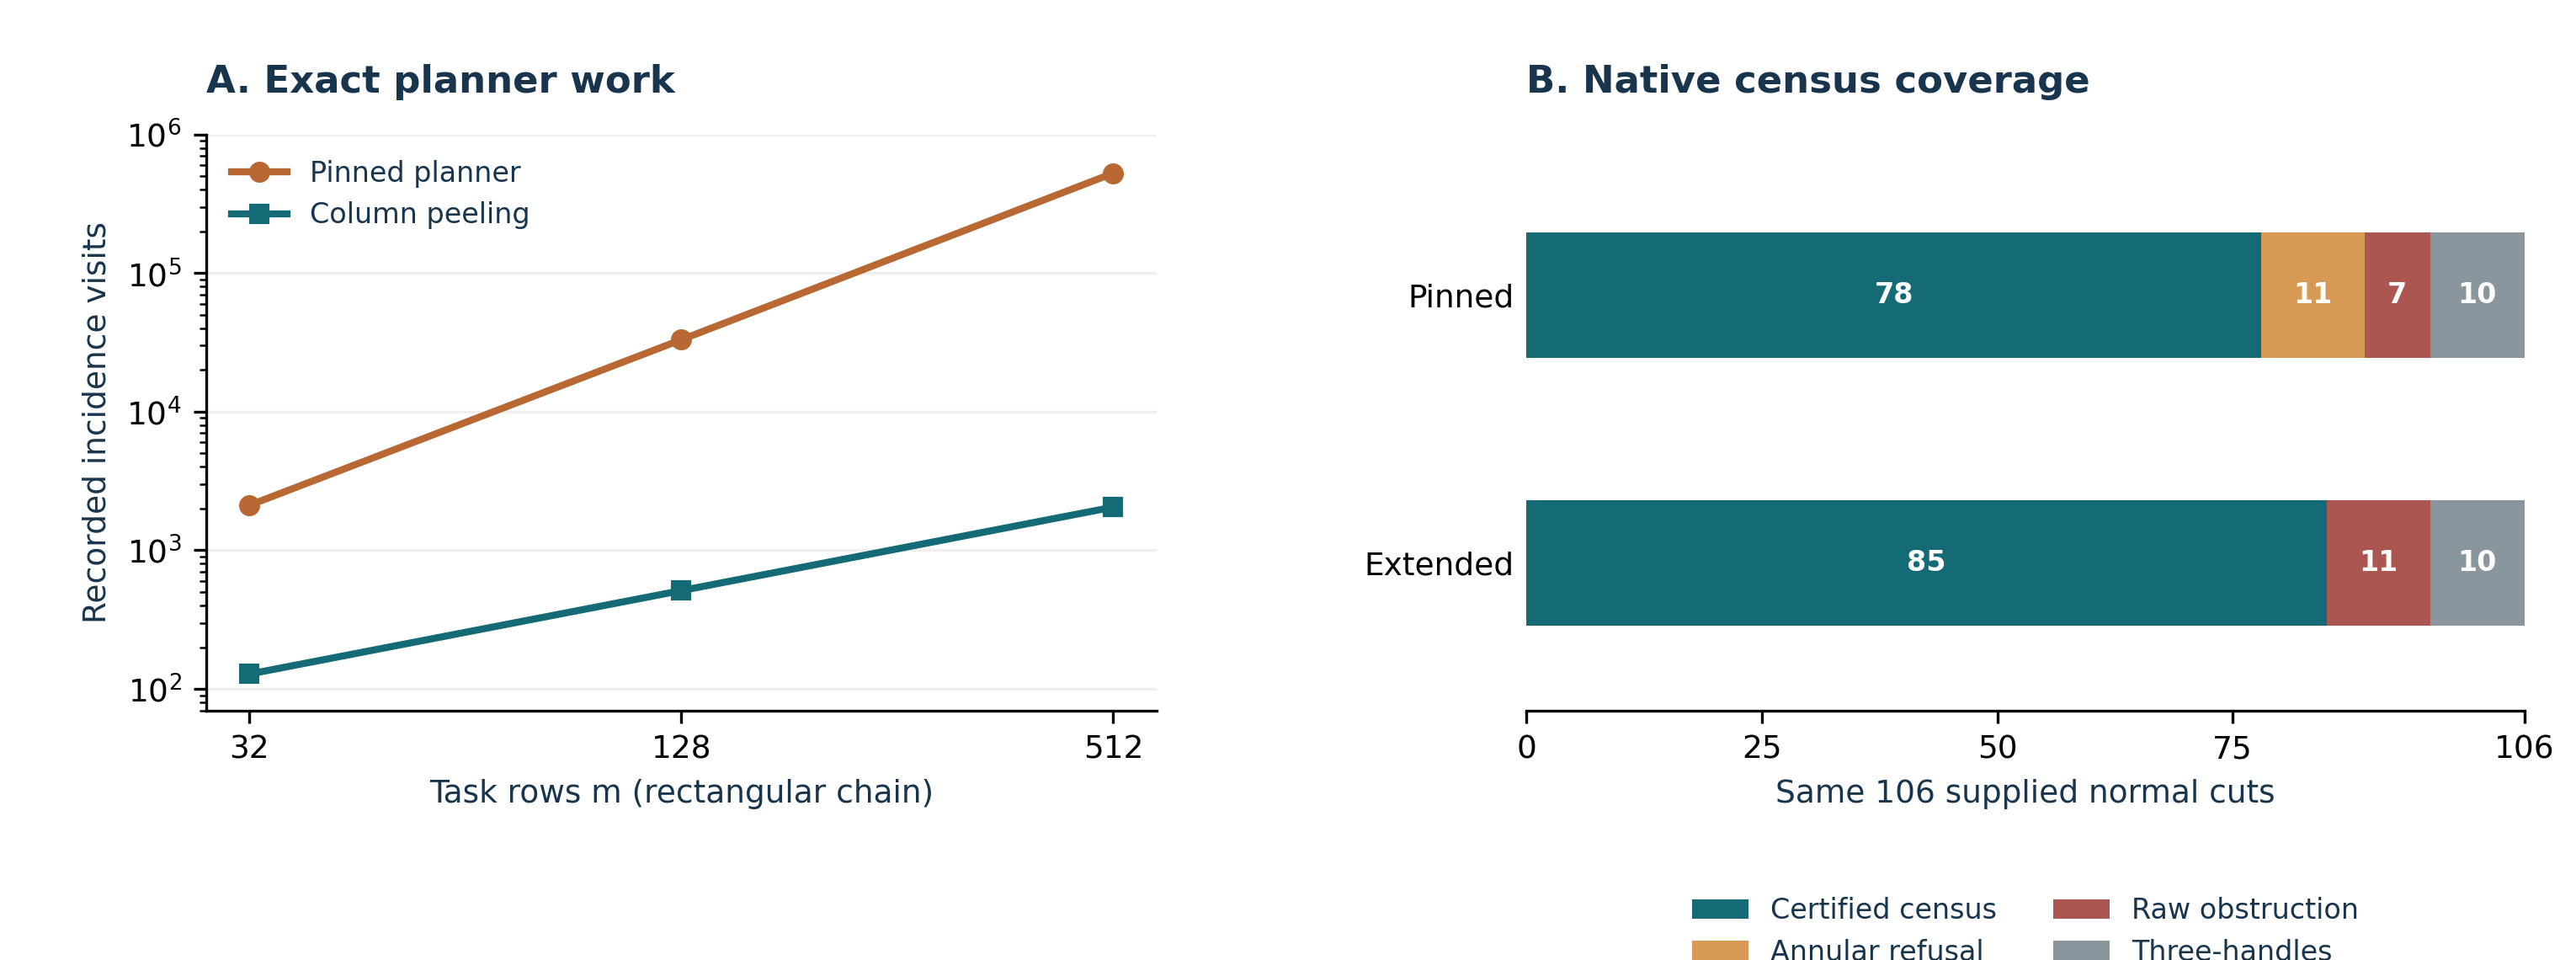
\includegraphics[width=\linewidth]{figures/work_and_coverage.png}
\caption{Left: exact recorded incidence work on rectangular chains,
including both source and deletion visits for the new method.  Right:
complete classification of the same 106 native source cases by each
consumer.  Numerical speedups on the left and topological coverage on the
right measure different improvements.}
\label{fig:work-coverage}
\end{figure}

The paired kernel timings used seven alternating-order rounds, with
separate A/A repetitions of the unchanged baseline and independent replay
timed separately.  They ran after the baseline regression process had
exited.  The following 128-row samples had comparatively stable controls.

\begin{table}[htbp]
\centering\small
\begin{tabular}{@{}lrrrr@{}}
\toprule
128-row family & Old ms & New ms & Old/new & A/A\\
\midrule
Rectangular chain & 8.424 & 0.293 & 28.73 & 1.004\\
Rectangular fan & 7.477 & 0.269 & 27.78 & 1.001\\
Cyclic stopping core & 5.075 & 0.102 & 49.73 & 1.024\\
\bottomrule
\end{tabular}
\caption{Medians for the planner kernel on Python 3.12.14.  Source-matrix
construction and JSON output are untimed.  Full raw samples and the
separate verifier times are preserved.}
\end{table}

The 512-row timing ratios are also retained, but their A/A controls range
from 1.070 to 1.194.  That variation is why exact work counts, rather than
the largest wall-time ratios, carry the asymptotic conclusion.

\subsection{Complete native calls and the optional precheck}

The whole-cut timings include source reconstruction.  In the verified
task, each repetition creates a fresh certificate and independently replays
it.  Module import, corpus-file loading, and JSON output are excluded.
All calls ran sequentially after the audits had finished; seven alternating
rounds and A/A controls were used.  The controls measure variability in
this shared execution environment, rather than claiming dedicated hardware.

\begin{table}[htbp]
\centering\small
\begin{tabularx}{\linewidth}{@{}Yrrrr@{}}
\toprule
Verified common-success task & Old ms & New ms & Old/new & A/A\\
\midrule
\texttt{pilot/fibonacci\_lst\_01/0} & 1.952 & 1.866 & 1.046 & 0.943\\
\texttt{fibonacci\_lst\_05/mixed} & 107.069 & 104.351 & 1.026 & 0.960\\
\texttt{relabel/4/0} & 432.042 & 444.604 & 0.972 & 1.003\\
\texttt{binary/1/500} & 7.438 & 7.726 & 0.963 & 1.011\\
\bottomrule
\end{tabularx}
\caption{The old and new consumers perform the same complete census task.
The final two rows are regressions in this sample.  Source discovery and
source replay dominate these small active matrices.}
\end{table}

These common-success measurements do not support a broad end-to-end speedup
claim.  The verified ratios range from 0.963 to 1.046, and several controls
show comparable variability.  The gain in positive coverage is the new
geometric construction, while the large kernel ratios apply to growing
incidence families rather than every native input.

The optional precheck gives a different, direct whole-call improvement.
On all 106 inputs it preserves the 85 successful certificates exactly.
It produces six early original-core obstruction proofs.  Five inputs
actually avoid two boundary orbit queries each, for ten avoided queries
in total.  The sixth, \texttt{pilot/finite\_trefoil/0}, has no ports, so
the original boundary stage already made zero orbit queries; only later
finite work is skipped there.

\begin{table}[htbp]
\centering\small
\begin{tabularx}{\linewidth}{@{}Yrrrr@{}}
\toprule
Verified obstruction task & Full path ms & Precheck ms & Ratio & A/A\\
\midrule
\texttt{pilot/fibonacci\_lst\_04/0} & 49.713 & 21.953 & 2.265 & 0.910\\
\texttt{pilot/fibonacci\_lst\_10/0} & 97.903 & 51.890 & 1.887 & 1.002\\
\texttt{pilot/lst\_4\_9/0} & 32.936 & 16.124 & 2.043 & 0.989\\
\texttt{pilot/finite\_trefoil/0} & 5.137 & 2.866 & 1.792 & 0.981\\
\bottomrule
\end{tabularx}
\caption{Equivalent refusal of this raw certificate method.  The early
proof establishes an original-core stopping subset and avoids compiling
the full residual matrix; it does not claim to output that matrix's
canonical residual.  The first A/A control is noticeably less stable.}
\end{table}

The stopping-set theorem justifies the skipped work.  Thus the two-query
savings are exact and the roughly twofold verified-call reductions in
these samples have an identified cause.  They remain measurements of
supplied-cut tasks, not of a complete unknot recognizer or a distribution
of arbitrary knot diagrams.
